\begin{figure}[htbp]
\centering
\begin{tikzpicture}
\begin{axis}[
    width=\columnwidth,
    height=0.6\textheight,
    xlabel={Frequency (Hz)},
    ylabel={Studies},
    xmode=log,
    log basis x=10,
    grid=major,
    grid style={dashed,gray!30},
    tick style={font=\footnotesize},
    label style={font=\small},
    title style={font=\normalsize},
    title={Band-pass Filter Frequency Ranges Across Studies},
    ytick={0,1,2,3,4,5,6,7,8,9,10,11,12,13,14,15,16,17,18,19,20,21,22,23,24,25,26,27,28,29,30,31,32,33,34,35,36,37,38,39,40,41,42,43,44,45,46,47,48,49,50,51,52,53,54,55,56,57,58,59},
    yticklabels={\cite{yeoInvestigatingCorticalActivity2024},\cite{chiossiMindVisualDiscomfort2024},\cite{mawalidClassificationEEGSignal2018},\cite{uyanCDMSRealtimeSystem2024},\cite{suwandiElectroencephalographySignalAnalysis2023},\cite{dennisonImprovingMotionSickness2019},\cite{liRestingstateEEGVestibular2023},\cite{mimnaughVirtualRealitySickness2023},\cite{liVRMotionSickness2020},\cite{andrievskaiaExploringNeurophysiologicalCorrelates2023},\cite{zhouApplicationEEGSTransformation2023},\cite{bergerSexDifferencesUser2021},\cite{wuInhibitionrelatedN2P32020},\cite{recentiPredictingMotionSickness2021},\cite{liExploringNeuralBiomarkers2023},\cite{liComparingAutonomicPhysiological2021},\cite{namElectroencephalogramMicrostatesFunctional2022},\cite{paneIdentifyingSeverityLevel2018},\cite{shenClassificationVisuallyInduced2024},\cite{huaAssessmentVirtualReality2023},\cite{moinnereauCybersicknessMarkerPrediction2024},\cite{chaiEEGStudyVirtual2023},\cite{khaitamiEEGVisualizationCybersickness2019},\cite{ozkanEffectsSpeedComplexity2023},\cite{jeongCybersicknessAnalysisEEG2019},\cite{kimPsychophysiologicalChangesNavigation2001},\cite{lin653QuantizationCybersickness2018},\cite{jangEstimatingObjectiveEEG2022},\cite{argasinskiElectroencephalographicEEGCorrelates2023},\cite{wooRecoveryTimeVR2023},\cite{limTestretestReliabilityVirtual2021},\cite{luoFeatureExtractionMethod2024},\cite{fengComprehensiveExplorationMotion2025},\cite{liuExploringQuantitativeAssessment2024},\cite{liuExploringBrainPhysiological2024},\cite{leeAssessingIndividualVR2022},\cite{yeoEEGbasedAnalysisVarious2022},\cite{chenSpatialTemporalEEG2010},\cite{linEEGEffectsMotion2007},\cite{krokosQuantifyingVRCybersickness2022},\cite{linMotionSicknessEstimation2012},\cite{chenMotionSicknessRelatedBrain2009},\cite{xuSECNNAttentionStructure2023},\cite{balajiNeurodynamicMappingCybersickness2025},\cite{koEEGbasedMotionSickness2013},\cite{nurnbergerMismatchVisualVestibularInformation2021},\cite{huaDetectionVirtualReality2024},\cite{weiEEGbasedEvaluationSystem2011},\cite{koEstimatingLevelMotion2011},\cite{ahnTemporalDynamicsVisually2020},\cite{huaSiamLSTMModelMultichannel2024},\cite{bergerInfluencePlaceboTDCS2024},\cite{bergerManipulatingCybersicknessVirtual2025},\cite{changEffectsRestFrames2013},\cite{kimDeepCybersicknessPredictor2019},\cite{huaEEGClassificationModel2024},\cite{huaDualpathwayEEGModel2025},\cite{suwandiExploringImpactMotion2024},\cite{changIdentifyingPhysiologicalCorrelates2022},\cite{kimCharacteristicChangesPhysiological2005}},
    yticklabel style={font=\tiny},
    xmin=0.1,
    xmax=105.0,
    enlarge y limits=0.05,
    legend pos=north west,
    legend style={font=\tiny},
]

% Center frequency points
\addplot[only marks, mark=*, mark size=2pt, black] coordinates {
    (0.1005, 0)
    (8.0, 1)
    (14.0, 2)
    (14.5, 3)
    (14.5, 4)
    (15.05, 5)
    (15.05, 6)
    (15.1, 7)
    (15.25, 8)
    (15.5, 9)
    (16.0, 10)
    (17.0, 11)
    (17.55, 12)
    (20.05, 13)
    (20.05, 14)
    (20.05, 15)
    (20.5, 16)
    (20.5, 17)
    (22.75, 18)
    (22.75, 19)
    (22.75, 20)
    (22.75, 21)
    (23.0, 22)
    (24.5, 23)
    (24.5, 24)
    (25.0, 25)
    (25.0, 26)
    (25.05, 27)
    (25.05, 28)
    (25.25, 29)
    (25.25, 30)
    (25.25, 31)
    (25.25, 32)
    (25.25, 33)
    (25.25, 34)
    (25.25, 35)
    (25.5, 36)
    (25.5, 37)
    (25.5, 38)
    (25.5, 39)
    (25.5, 40)
    (25.5, 41)
    (25.5, 42)
    (25.5, 43)
    (25.5, 44)
    (30.05, 45)
    (30.25, 46)
    (30.5, 47)
    (30.5, 48)
    (35.05, 49)
    (40.25, 50)
    (50.005, 51)
    (50.05, 52)
    (50.05, 53)
    (50.15, 54)
    (50.25, 55)
    (50.25, 56)
    (50.25, 57)
    (50.25, 58)
    (50.5, 59)
};
\addlegendentry{Center frequency}

% Frequency range bars (low-high)
\draw[black, line width=1.5pt] (axis cs:0.001,0) -- (axis cs:0.2,0);
\draw[black, line width=1.5pt] (axis cs:0.001,-0.15) -- (axis cs:0.001,0.15);
\draw[black, line width=1.5pt] (axis cs:0.2,-0.15) -- (axis cs:0.2,0.15);
\draw[black, line width=1.5pt] (axis cs:1.0,1) -- (axis cs:15.0,1);
\draw[black, line width=1.5pt] (axis cs:1.0,0.85) -- (axis cs:1.0,1.15);
\draw[black, line width=1.5pt] (axis cs:15.0,0.85) -- (axis cs:15.0,1.15);
\draw[black, line width=1.5pt] (axis cs:8.0,2) -- (axis cs:20.0,2);
\draw[black, line width=1.5pt] (axis cs:8.0,1.85) -- (axis cs:8.0,2.15);
\draw[black, line width=1.5pt] (axis cs:20.0,1.85) -- (axis cs:20.0,2.15);
\draw[black, line width=1.5pt] (axis cs:4.0,3) -- (axis cs:25.0,3);
\draw[black, line width=1.5pt] (axis cs:4.0,2.85) -- (axis cs:4.0,3.15);
\draw[black, line width=1.5pt] (axis cs:25.0,2.85) -- (axis cs:25.0,3.15);
\draw[black, line width=1.5pt] (axis cs:8.0,4) -- (axis cs:21.0,4);
\draw[black, line width=1.5pt] (axis cs:8.0,3.85) -- (axis cs:8.0,4.15);
\draw[black, line width=1.5pt] (axis cs:21.0,3.85) -- (axis cs:21.0,4.15);
\draw[black, line width=1.5pt] (axis cs:0.1,5) -- (axis cs:30.0,5);
\draw[black, line width=1.5pt] (axis cs:0.1,4.85) -- (axis cs:0.1,5.15);
\draw[black, line width=1.5pt] (axis cs:30.0,4.85) -- (axis cs:30.0,5.15);
\draw[black, line width=1.5pt] (axis cs:0.1,6) -- (axis cs:30.0,6);
\draw[black, line width=1.5pt] (axis cs:0.1,5.85) -- (axis cs:0.1,6.15);
\draw[black, line width=1.5pt] (axis cs:30.0,5.85) -- (axis cs:30.0,6.15);
\draw[black, line width=1.5pt] (axis cs:0.2,7) -- (axis cs:30.0,7);
\draw[black, line width=1.5pt] (axis cs:0.2,6.85) -- (axis cs:0.2,7.15);
\draw[black, line width=1.5pt] (axis cs:30.0,6.85) -- (axis cs:30.0,7.15);
\draw[black, line width=1.5pt] (axis cs:0.5,8) -- (axis cs:30.0,8);
\draw[black, line width=1.5pt] (axis cs:0.5,7.85) -- (axis cs:0.5,8.15);
\draw[black, line width=1.5pt] (axis cs:30.0,7.85) -- (axis cs:30.0,8.15);
\draw[black, line width=1.5pt] (axis cs:1.0,9) -- (axis cs:30.0,9);
\draw[black, line width=1.5pt] (axis cs:1.0,8.85) -- (axis cs:1.0,9.15);
\draw[black, line width=1.5pt] (axis cs:30.0,8.85) -- (axis cs:30.0,9.15);
\draw[black, line width=1.5pt] (axis cs:0.0,10) -- (axis cs:32.0,10);
\draw[black, line width=1.5pt] (axis cs:0.0,9.85) -- (axis cs:0.0,10.15);
\draw[black, line width=1.5pt] (axis cs:32.0,9.85) -- (axis cs:32.0,10.15);
\draw[black, line width=1.5pt] (axis cs:4.0,11) -- (axis cs:30.0,11);
\draw[black, line width=1.5pt] (axis cs:4.0,10.85) -- (axis cs:4.0,11.15);
\draw[black, line width=1.5pt] (axis cs:30.0,10.85) -- (axis cs:30.0,11.15);
\draw[black, line width=1.5pt] (axis cs:0.1,12) -- (axis cs:35.0,12);
\draw[black, line width=1.5pt] (axis cs:0.1,11.85) -- (axis cs:0.1,12.15);
\draw[black, line width=1.5pt] (axis cs:35.0,11.85) -- (axis cs:35.0,12.15);
\draw[black, line width=1.5pt] (axis cs:0.1,13) -- (axis cs:40.0,13);
\draw[black, line width=1.5pt] (axis cs:0.1,12.85) -- (axis cs:0.1,13.15);
\draw[black, line width=1.5pt] (axis cs:40.0,12.85) -- (axis cs:40.0,13.15);
\draw[black, line width=1.5pt] (axis cs:0.1,14) -- (axis cs:40.0,14);
\draw[black, line width=1.5pt] (axis cs:0.1,13.85) -- (axis cs:0.1,14.15);
\draw[black, line width=1.5pt] (axis cs:40.0,13.85) -- (axis cs:40.0,14.15);
\draw[black, line width=1.5pt] (axis cs:0.1,15) -- (axis cs:40.0,15);
\draw[black, line width=1.5pt] (axis cs:0.1,14.85) -- (axis cs:0.1,15.15);
\draw[black, line width=1.5pt] (axis cs:40.0,14.85) -- (axis cs:40.0,15.15);
\draw[black, line width=1.5pt] (axis cs:1.0,16) -- (axis cs:40.0,16);
\draw[black, line width=1.5pt] (axis cs:1.0,15.85) -- (axis cs:1.0,16.15);
\draw[black, line width=1.5pt] (axis cs:40.0,15.85) -- (axis cs:40.0,16.15);
\draw[black, line width=1.5pt] (axis cs:1.0,17) -- (axis cs:40.0,17);
\draw[black, line width=1.5pt] (axis cs:1.0,16.85) -- (axis cs:1.0,17.15);
\draw[black, line width=1.5pt] (axis cs:40.0,16.85) -- (axis cs:40.0,17.15);
\draw[black, line width=1.5pt] (axis cs:0.5,18) -- (axis cs:45.0,18);
\draw[black, line width=1.5pt] (axis cs:0.5,17.85) -- (axis cs:0.5,18.15);
\draw[black, line width=1.5pt] (axis cs:45.0,17.85) -- (axis cs:45.0,18.15);
\draw[black, line width=1.5pt] (axis cs:0.5,19) -- (axis cs:45.0,19);
\draw[black, line width=1.5pt] (axis cs:0.5,18.85) -- (axis cs:0.5,19.15);
\draw[black, line width=1.5pt] (axis cs:45.0,18.85) -- (axis cs:45.0,19.15);
\draw[black, line width=1.5pt] (axis cs:0.5,20) -- (axis cs:45.0,20);
\draw[black, line width=1.5pt] (axis cs:0.5,19.85) -- (axis cs:0.5,20.15);
\draw[black, line width=1.5pt] (axis cs:45.0,19.85) -- (axis cs:45.0,20.15);
\draw[black, line width=1.5pt] (axis cs:0.5,21) -- (axis cs:45.0,21);
\draw[black, line width=1.5pt] (axis cs:0.5,20.85) -- (axis cs:0.5,21.15);
\draw[black, line width=1.5pt] (axis cs:45.0,20.85) -- (axis cs:45.0,21.15);
\draw[black, line width=1.5pt] (axis cs:1.0,22) -- (axis cs:45.0,22);
\draw[black, line width=1.5pt] (axis cs:1.0,21.85) -- (axis cs:1.0,22.15);
\draw[black, line width=1.5pt] (axis cs:45.0,21.85) -- (axis cs:45.0,22.15);
\draw[black, line width=1.5pt] (axis cs:1.0,23) -- (axis cs:48.0,23);
\draw[black, line width=1.5pt] (axis cs:1.0,22.85) -- (axis cs:1.0,23.15);
\draw[black, line width=1.5pt] (axis cs:48.0,22.85) -- (axis cs:48.0,23.15);
\draw[black, line width=1.5pt] (axis cs:4.0,24) -- (axis cs:45.0,24);
\draw[black, line width=1.5pt] (axis cs:4.0,23.85) -- (axis cs:4.0,24.15);
\draw[black, line width=1.5pt] (axis cs:45.0,23.85) -- (axis cs:45.0,24.15);
\draw[black, line width=1.5pt] (axis cs:0.0,25) -- (axis cs:50.0,25);
\draw[black, line width=1.5pt] (axis cs:0.0,24.85) -- (axis cs:0.0,25.15);
\draw[black, line width=1.5pt] (axis cs:50.0,24.85) -- (axis cs:50.0,25.15);
\draw[black, line width=1.5pt] (axis cs:0.0,26) -- (axis cs:50.0,26);
\draw[black, line width=1.5pt] (axis cs:0.0,25.85) -- (axis cs:0.0,26.15);
\draw[black, line width=1.5pt] (axis cs:50.0,25.85) -- (axis cs:50.0,26.15);
\draw[black, line width=1.5pt] (axis cs:0.1,27) -- (axis cs:50.0,27);
\draw[black, line width=1.5pt] (axis cs:0.1,26.85) -- (axis cs:0.1,27.15);
\draw[black, line width=1.5pt] (axis cs:50.0,26.85) -- (axis cs:50.0,27.15);
\draw[black, line width=1.5pt] (axis cs:0.1,28) -- (axis cs:50.0,28);
\draw[black, line width=1.5pt] (axis cs:0.1,27.85) -- (axis cs:0.1,28.15);
\draw[black, line width=1.5pt] (axis cs:50.0,27.85) -- (axis cs:50.0,28.15);
\draw[black, line width=1.5pt] (axis cs:0.5,29) -- (axis cs:50.0,29);
\draw[black, line width=1.5pt] (axis cs:0.5,28.85) -- (axis cs:0.5,29.15);
\draw[black, line width=1.5pt] (axis cs:50.0,28.85) -- (axis cs:50.0,29.15);
\draw[black, line width=1.5pt] (axis cs:0.5,30) -- (axis cs:50.0,30);
\draw[black, line width=1.5pt] (axis cs:0.5,29.85) -- (axis cs:0.5,30.15);
\draw[black, line width=1.5pt] (axis cs:50.0,29.85) -- (axis cs:50.0,30.15);
\draw[black, line width=1.5pt] (axis cs:0.5,31) -- (axis cs:50.0,31);
\draw[black, line width=1.5pt] (axis cs:0.5,30.85) -- (axis cs:0.5,31.15);
\draw[black, line width=1.5pt] (axis cs:50.0,30.85) -- (axis cs:50.0,31.15);
\draw[black, line width=1.5pt] (axis cs:0.5,32) -- (axis cs:50.0,32);
\draw[black, line width=1.5pt] (axis cs:0.5,31.85) -- (axis cs:0.5,32.15);
\draw[black, line width=1.5pt] (axis cs:50.0,31.85) -- (axis cs:50.0,32.15);
\draw[black, line width=1.5pt] (axis cs:0.5,33) -- (axis cs:50.0,33);
\draw[black, line width=1.5pt] (axis cs:0.5,32.85) -- (axis cs:0.5,33.15);
\draw[black, line width=1.5pt] (axis cs:50.0,32.85) -- (axis cs:50.0,33.15);
\draw[black, line width=1.5pt] (axis cs:0.5,34) -- (axis cs:50.0,34);
\draw[black, line width=1.5pt] (axis cs:0.5,33.85) -- (axis cs:0.5,34.15);
\draw[black, line width=1.5pt] (axis cs:50.0,33.85) -- (axis cs:50.0,34.15);
\draw[black, line width=1.5pt] (axis cs:0.5,35) -- (axis cs:50.0,35);
\draw[black, line width=1.5pt] (axis cs:0.5,34.85) -- (axis cs:0.5,35.15);
\draw[black, line width=1.5pt] (axis cs:50.0,34.85) -- (axis cs:50.0,35.15);
\draw[black, line width=1.5pt] (axis cs:1.0,36) -- (axis cs:50.0,36);
\draw[black, line width=1.5pt] (axis cs:1.0,35.85) -- (axis cs:1.0,36.15);
\draw[black, line width=1.5pt] (axis cs:50.0,35.85) -- (axis cs:50.0,36.15);
\draw[black, line width=1.5pt] (axis cs:1.0,37) -- (axis cs:50.0,37);
\draw[black, line width=1.5pt] (axis cs:1.0,36.85) -- (axis cs:1.0,37.15);
\draw[black, line width=1.5pt] (axis cs:50.0,36.85) -- (axis cs:50.0,37.15);
\draw[black, line width=1.5pt] (axis cs:1.0,38) -- (axis cs:50.0,38);
\draw[black, line width=1.5pt] (axis cs:1.0,37.85) -- (axis cs:1.0,38.15);
\draw[black, line width=1.5pt] (axis cs:50.0,37.85) -- (axis cs:50.0,38.15);
\draw[black, line width=1.5pt] (axis cs:1.0,39) -- (axis cs:50.0,39);
\draw[black, line width=1.5pt] (axis cs:1.0,38.85) -- (axis cs:1.0,39.15);
\draw[black, line width=1.5pt] (axis cs:50.0,38.85) -- (axis cs:50.0,39.15);
\draw[black, line width=1.5pt] (axis cs:1.0,40) -- (axis cs:50.0,40);
\draw[black, line width=1.5pt] (axis cs:1.0,39.85) -- (axis cs:1.0,40.15);
\draw[black, line width=1.5pt] (axis cs:50.0,39.85) -- (axis cs:50.0,40.15);
\draw[black, line width=1.5pt] (axis cs:1.0,41) -- (axis cs:50.0,41);
\draw[black, line width=1.5pt] (axis cs:1.0,40.85) -- (axis cs:1.0,41.15);
\draw[black, line width=1.5pt] (axis cs:50.0,40.85) -- (axis cs:50.0,41.15);
\draw[black, line width=1.5pt] (axis cs:1.0,42) -- (axis cs:50.0,42);
\draw[black, line width=1.5pt] (axis cs:1.0,41.85) -- (axis cs:1.0,42.15);
\draw[black, line width=1.5pt] (axis cs:50.0,41.85) -- (axis cs:50.0,42.15);
\draw[black, line width=1.5pt] (axis cs:1.0,43) -- (axis cs:50.0,43);
\draw[black, line width=1.5pt] (axis cs:1.0,42.85) -- (axis cs:1.0,43.15);
\draw[black, line width=1.5pt] (axis cs:50.0,42.85) -- (axis cs:50.0,43.15);
\draw[black, line width=1.5pt] (axis cs:1.0,44) -- (axis cs:50.0,44);
\draw[black, line width=1.5pt] (axis cs:1.0,43.85) -- (axis cs:1.0,44.15);
\draw[black, line width=1.5pt] (axis cs:50.0,43.85) -- (axis cs:50.0,44.15);
\draw[black, line width=1.5pt] (axis cs:0.1,45) -- (axis cs:60.0,45);
\draw[black, line width=1.5pt] (axis cs:0.1,44.85) -- (axis cs:0.1,45.15);
\draw[black, line width=1.5pt] (axis cs:60.0,44.85) -- (axis cs:60.0,45.15);
\draw[black, line width=1.5pt] (axis cs:0.5,46) -- (axis cs:60.0,46);
\draw[black, line width=1.5pt] (axis cs:0.5,45.85) -- (axis cs:0.5,46.15);
\draw[black, line width=1.5pt] (axis cs:60.0,45.85) -- (axis cs:60.0,46.15);
\draw[black, line width=1.5pt] (axis cs:1.0,47) -- (axis cs:60.0,47);
\draw[black, line width=1.5pt] (axis cs:1.0,46.85) -- (axis cs:1.0,47.15);
\draw[black, line width=1.5pt] (axis cs:60.0,46.85) -- (axis cs:60.0,47.15);
\draw[black, line width=1.5pt] (axis cs:1.0,48) -- (axis cs:60.0,48);
\draw[black, line width=1.5pt] (axis cs:1.0,47.85) -- (axis cs:1.0,48.15);
\draw[black, line width=1.5pt] (axis cs:60.0,47.85) -- (axis cs:60.0,48.15);
\draw[black, line width=1.5pt] (axis cs:0.1,49) -- (axis cs:70.0,49);
\draw[black, line width=1.5pt] (axis cs:0.1,48.85) -- (axis cs:0.1,49.15);
\draw[black, line width=1.5pt] (axis cs:70.0,48.85) -- (axis cs:70.0,49.15);
\draw[black, line width=1.5pt] (axis cs:0.5,50) -- (axis cs:80.0,50);
\draw[black, line width=1.5pt] (axis cs:0.5,49.85) -- (axis cs:0.5,50.15);
\draw[black, line width=1.5pt] (axis cs:80.0,49.85) -- (axis cs:80.0,50.15);
\draw[black, line width=1.5pt] (axis cs:0.01,51) -- (axis cs:100.0,51);
\draw[black, line width=1.5pt] (axis cs:0.01,50.85) -- (axis cs:0.01,51.15);
\draw[black, line width=1.5pt] (axis cs:100.0,50.85) -- (axis cs:100.0,51.15);
\draw[black, line width=1.5pt] (axis cs:0.1,52) -- (axis cs:100.0,52);
\draw[black, line width=1.5pt] (axis cs:0.1,51.85) -- (axis cs:0.1,52.15);
\draw[black, line width=1.5pt] (axis cs:100.0,51.85) -- (axis cs:100.0,52.15);
\draw[black, line width=1.5pt] (axis cs:0.1,53) -- (axis cs:100.0,53);
\draw[black, line width=1.5pt] (axis cs:0.1,52.85) -- (axis cs:0.1,53.15);
\draw[black, line width=1.5pt] (axis cs:100.0,52.85) -- (axis cs:100.0,53.15);
\draw[black, line width=1.5pt] (axis cs:0.3,54) -- (axis cs:100.0,54);
\draw[black, line width=1.5pt] (axis cs:0.3,53.85) -- (axis cs:0.3,54.15);
\draw[black, line width=1.5pt] (axis cs:100.0,53.85) -- (axis cs:100.0,54.15);
\draw[black, line width=1.5pt] (axis cs:0.5,55) -- (axis cs:100.0,55);
\draw[black, line width=1.5pt] (axis cs:0.5,54.85) -- (axis cs:0.5,55.15);
\draw[black, line width=1.5pt] (axis cs:100.0,54.85) -- (axis cs:100.0,55.15);
\draw[black, line width=1.5pt] (axis cs:0.5,56) -- (axis cs:100.0,56);
\draw[black, line width=1.5pt] (axis cs:0.5,55.85) -- (axis cs:0.5,56.15);
\draw[black, line width=1.5pt] (axis cs:100.0,55.85) -- (axis cs:100.0,56.15);
\draw[black, line width=1.5pt] (axis cs:0.5,57) -- (axis cs:100.0,57);
\draw[black, line width=1.5pt] (axis cs:0.5,56.85) -- (axis cs:0.5,57.15);
\draw[black, line width=1.5pt] (axis cs:100.0,56.85) -- (axis cs:100.0,57.15);
\draw[black, line width=1.5pt] (axis cs:0.5,58) -- (axis cs:100.0,58);
\draw[black, line width=1.5pt] (axis cs:0.5,57.85) -- (axis cs:0.5,58.15);
\draw[black, line width=1.5pt] (axis cs:100.0,57.85) -- (axis cs:100.0,58.15);
\draw[black, line width=1.5pt] (axis cs:1.0,59) -- (axis cs:100.0,59);
\draw[black, line width=1.5pt] (axis cs:1.0,58.85) -- (axis cs:1.0,59.15);
\draw[black, line width=1.5pt] (axis cs:100.0,58.85) -- (axis cs:100.0,59.15);

% Notch filter crosses
\draw[red, line width=1.5pt] (axis cs:50.0,0.8) -- (axis cs:50.0,1.2);
\draw[red, line width=1.5pt] (axis cs:47.5,1) -- (axis cs:52.5,1);
\draw[red, line width=1.5pt] (axis cs:60.0,3.8) -- (axis cs:60.0,4.2);
\draw[red, line width=1.5pt] (axis cs:57.0,4) -- (axis cs:63.0,4);
\draw[red, line width=1.5pt] (axis cs:50.0,17.8) -- (axis cs:50.0,18.2);
\draw[red, line width=1.5pt] (axis cs:47.5,18) -- (axis cs:52.5,18);
\draw[red, line width=1.5pt] (axis cs:50.0,18.8) -- (axis cs:50.0,19.2);
\draw[red, line width=1.5pt] (axis cs:47.5,19) -- (axis cs:52.5,19);
\draw[red, line width=1.5pt] (axis cs:50.0,20.8) -- (axis cs:50.0,21.2);
\draw[red, line width=1.5pt] (axis cs:47.5,21) -- (axis cs:52.5,21);
\draw[red, line width=1.5pt] (axis cs:50.0,22.8) -- (axis cs:50.0,23.2);
\draw[red, line width=1.5pt] (axis cs:47.5,23) -- (axis cs:52.5,23);
\draw[red, line width=1.5pt] (axis cs:50.0,27.8) -- (axis cs:50.0,28.2);
\draw[red, line width=1.5pt] (axis cs:47.5,28) -- (axis cs:52.5,28);
\draw[red, line width=1.5pt] (axis cs:60.0,28.8) -- (axis cs:60.0,29.2);
\draw[red, line width=1.5pt] (axis cs:57.0,29) -- (axis cs:63.0,29);
\draw[red, line width=1.5pt] (axis cs:50.0,41.8) -- (axis cs:50.0,42.2);
\draw[red, line width=1.5pt] (axis cs:47.5,42) -- (axis cs:52.5,42);
\draw[red, line width=1.5pt] (axis cs:50.0,45.8) -- (axis cs:50.0,46.2);
\draw[red, line width=1.5pt] (axis cs:47.5,46) -- (axis cs:52.5,46);
\draw[red, line width=1.5pt] (axis cs:50.0,49.8) -- (axis cs:50.0,50.2);
\draw[red, line width=1.5pt] (axis cs:47.5,50) -- (axis cs:52.5,50);
\draw[red, line width=1.5pt] (axis cs:50.0,50.8) -- (axis cs:50.0,51.2);
\draw[red, line width=1.5pt] (axis cs:47.5,51) -- (axis cs:52.5,51);
\draw[red, line width=1.5pt] (axis cs:50.0,51.8) -- (axis cs:50.0,52.2);
\draw[red, line width=1.5pt] (axis cs:47.5,52) -- (axis cs:52.5,52);
\draw[red, line width=1.5pt] (axis cs:60.0,53.8) -- (axis cs:60.0,54.2);
\draw[red, line width=1.5pt] (axis cs:57.0,54) -- (axis cs:63.0,54);
\draw[red, line width=1.5pt] (axis cs:50.0,54.8) -- (axis cs:50.0,55.2);
\draw[red, line width=1.5pt] (axis cs:47.5,55) -- (axis cs:52.5,55);
\draw[red, line width=1.5pt] (axis cs:50.0,55.8) -- (axis cs:50.0,56.2);
\draw[red, line width=1.5pt] (axis cs:47.5,56) -- (axis cs:52.5,56);
\draw[red, line width=1.5pt] (axis cs:60.0,57.8) -- (axis cs:60.0,58.2);
\draw[red, line width=1.5pt] (axis cs:57.0,58) -- (axis cs:63.0,58);
\draw[red, line width=1.5pt] (axis cs:60.0,58.8) -- (axis cs:60.0,59.2);
\draw[red, line width=1.5pt] (axis cs:57.0,59) -- (axis cs:63.0,59);

% Legend entries
\addlegendimage{black, line width=1.5pt}
\addlegendentry{Frequency range}
\addlegendimage{red, mark=x, mark size=3pt, only marks}
\addlegendentry{Notch filter}

\end{axis}
\end{tikzpicture}
\caption{Band-pass filter frequency ranges across studies showing center frequency (black dots) with frequency ranges (black error bars) and notch filter frequencies (red crosses). The frequency range shows the low and high cutoff frequencies of the band-pass filters, while red crosses indicate notch filter frequencies used to remove specific interference (e.g., 50/60 Hz power line noise).}
\label{fig:bandpass_distribution}
\end{figure}
